\documentclass[a4j,fleqn,10pt]{jarticle}

\usepackage{ipsj}
\usepackage{txfonts}
\usepackage[symbol*,perpage]{footmisc}
\usepackage[dvipdfmx]{graphicx}
\usepackage{graphicx}
\usepackage{otf}

\def\Maru#1{\textcircled{\scriptsize #1}}

\begin{document}

\jtitle{ダークネット観測結果による Hajime の Mirai に対する影響の調査}
\jcontact{防衛大学校 理工学研究科 サイバーセキュリティ工学}
\jauthor{ファン・アン・ソン\dag, \ \ \ \ 中村 康弘\ddag}

\maketitle

\footnotetext[0]{\hspace*{-6.5mm}A Survey of Hajime's Impact on Mirai from Darknet Observation,\\
\dag Son Pham Anh, \ddag Yasuhiro Nakamura,\\
Cyber Security Engineering, National Defense Academy}


%川野くんへ
% "%" でコメントする
% 段落と段落は改行で

\section{はじめに}
近年、IoT機器が急速に普及・発展しているが、同時に、それらを標的とする Mirai, Hajimeなどのワームの活動が活発化している。
%
Miraiは
ランダムな宛先IPアドレスを生成してパスワードの辞書攻撃により感染を拡大するとともに、
ボットネットを構築してC\&Cサーバからの指示によりDDoS攻撃を行うワームタイプのマルウェアである。
%
HajimeはMiraiと同じようにIoTデバイスへの感染を試みるが、
DDoS攻撃のようなサイバー攻撃の機能は搭載していない。
Hajime感染後はMiraiが感染拡大するためのポートを閉じることで
Miraiの感染を妨害すると報告されている。
%
これらのワームはIPアドレスをランダムに生成して感染を拡大しようとするため、
未使用アドレスのへ着信する接続要求パケットを観測することで、
これらの活動状況を把握することができる。



\section{関連研究}
MiraiとHajimeについては多くの研究や報告がなされている。
%
NICTはダークネットに到着したパケット数の観測結果を報告した\cite{nict18}。
このレポートではMirai, Hajimeの感染活動が観測された日時と送信者の国別統計を公表した。
また、1日ごとのユニークな送信元アドレス数の増減も報告した。
その結果、Hajimeの感染数はMiraiの感染数の数倍程度であることを示し、
HajimeとMiraiの感染の規模と感染活動が活性化した日が明らかとなった。
%
IIJ-SECセキュリティレポート2018\cite{iij-sec18}は、ハニーポートに到着したパケットを使用して、
Mirai, qBot, Hajimeの感染活動を調査した。
レポートではマルウェア感染活動の傾向を明らかにし、
各ポートの送信元IPアドレスの数を示した。
そして、2019のレポート\cite{iij-sec19}ではハニーポットで受信したパケットデータを元に、
Mirai, Hajimeの感染活動状況を調査し、Miraiの亜種の活動状況も調査した。
%


これらのレポートはMirai, Hajimeの通信特徴を持つパケットの送信元IPアドレスに着目し、
1日ごとのユニークな送信元アドレス数を計測することにより、感染活動を把握する。
ただし、この手法では新たに出現する送信元アドレス数と
回復した送信元アドレス数を把握することができないため、
新規感染数の増減が不明であった。
%

そこで本研究では、長期間にわたる
Mirai, Hajimeの新規出現送信元アドレス数と回復した送信元アドレス数を調査することで、
HajimeのMiraiに対する影響を明らかにする。
%


\section{調査方法}
この報告では、NICTが提供しているダークネット観測データセットのうち、
2016年1月1日から2018年12月31日までの3年間分を用いた。
%
ここで、Hajimeからの接続要求パケットはWindow Sizeが14600であること、
Miraiの接続要求パケットのシーケンス番号は宛先IPアドレスと同一であること\cite{nict18}
を条件とすることで、
感染活動を行なったIPアドレスとその活動日時を調査する。
%
長期にわたる観測結果に対してこの条件を処理を適用することで、
その日に新規に感染したアドレス数、接続要求が来なくなることで
回復したとみなすことができるアドレス数のそれぞれを調査することができる。


\begin{figure}[t]
\centering
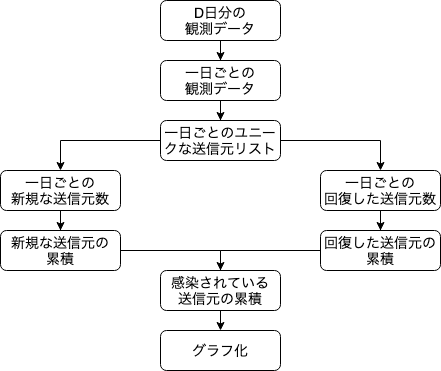
\includegraphics[width=7cm]{method_1.png}
\caption{処理手順}\label{method}
\end{figure}


\begin{figure*}[t]
\centering
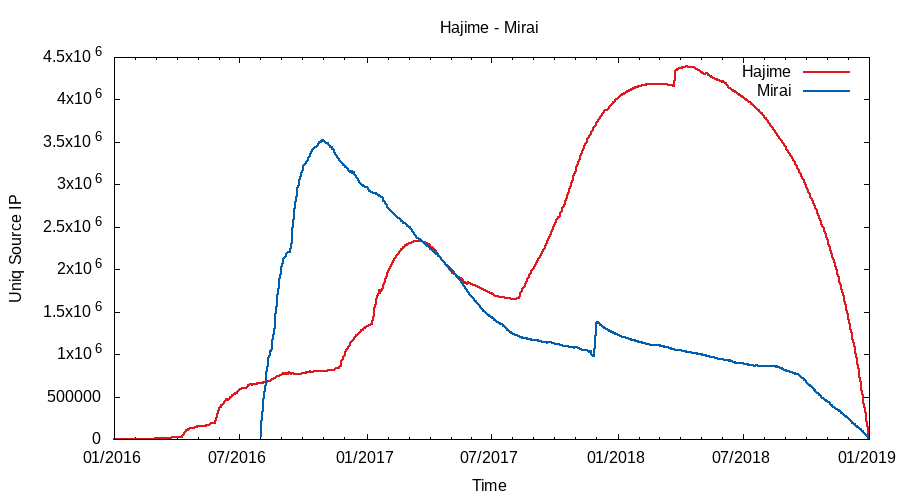
\includegraphics[width=14cm]{result.png}
\caption{Mirai, Hajimeの感染アドレス数の推移}\label{result}
\end{figure*}




\subsection{処理手順}
長期にわたる観測結果のデータを用いて、以下の処理を行う。

%本研究の実験手法は図\ref{method}のように6つのステップに分かれる。
%
\begin{description}
\vspace{-1.2ex}
\item{Step1:}
D日分の観測データを一日ごとに分割する。
%
\vspace{-1.2ex}
\item{Step2:}
一日ごとのデータに対して、Hajime, Miraiのそれぞれの特徴を持つ接続要求パケットを抽出し、
その送信元アドレスの重複を除いてユニークな送信元アドレスリスト$L_i$を作成する。
\vspace{-1.2ex}
%
\item{Step3:}
D日分の$L_i (i=1,...,D)$から一日ごとに新規に出現した送信元アドレス数 $N_i$ と
回復した送信元アドレス数 $R_i$ を求める。
%
\vspace{-1.2ex}
\item{Step4:}
新規な送信元アドレスと回復アドレスのそれぞれの累積を $TN_i, TR_i$ を集計する。
%
\vspace{-1.2ex}
\item{Step5:}
これらの差分により、その日に感染拡大活動を行なっているアドレス数 $K_i$ を求める。
\vspace{-1.2ex}
\begin{equation}
K_i = TN_i - TR_i
\end{equation}
%
\vspace{-1.2ex}
\item{Step6:}
得られた $K_i$ をグラフ表示することで実際の感染数の推移を可視化する。

\end{description}



\section{結果}
%
Mirai、Hajimeに感染されている送信元数の推移を図\ref{result}に示す。
%
Miraiの特徴を持ったパケットは2016年8月1日以前には存在せず、その日から急激に増大した。
Hajimeの特徴を持ったパケットは2016年8月1日以前にも存在していることが確認できた。
%
図\ref{result}を
時間軸方向に見るとHajimeの数が徐々に増えているが、その増加にともなって
Miraiの数が急速に減少していることがわかる。
%
これは、Hajimeが感染した機器は、Miraiが感染するためのポート番号を閉じることでMiraiの感染が妨害されたためと考えられる。
%
これらのワームはメモリ上で動作しており、機器の再起動により活動を停止する。
このため、同一アドレスから複数日にわたって継続的に感染活動があったアドレスに対して、
重複のないアドレス数および活動の継続日数を調査した。
その結果、
Miraiの特徴を持ったパケットの送信元アドレスの種類数は約3600万アドレスで、
それぞれのアドレスの平均生存時間は約38日間であった。
%
Hajimeの送信元アドレスの種類数は約2500万アドレスで、
平均生存時間はMiraiの約3倍の90日であった。
%


\section{まとめ}
%
従来の観測報告では1日毎の感染数のみに着目していたため、新規に感染した数が明らかではなかった。
これは長期にわたってユニークなアドレス数を求めるという負荷の大きい処理を必要とするためである。
%
この研究では特徴量によるフィルタリング処理とユニークなアドレスを抽出する処理を分離することで
新規に観測されたアドレスや現れなくなったアドレス等を求めることができるようになった。
%
この結果、Hajimeの感染拡大に伴ってMiraiの感染数が減少している状況を定量的に捉えることができた。
%
今後、処理のためのメモリ効率等について改善する必要がある。

%
%
\begin{thebibliography}{3}

\bibitem{nict18}
情報通信研究機構サイバーセキュリティ研究室, NICTER観測レポート2018年,
{\tt https://www.nict\\.go.jp/press/2019/02/06-1.html}, 2019.

\vspace{-1ex}
\bibitem{iij-sec18}
IIJ-SEC・Masafumi Negishi, 2018年のIoTボット観測状況と最近の動向,
{\tt https://sect.iij.ad.jp/d\\/2019/01/288147.html}, 2019.

\vspace{-1ex}
\bibitem{iij-sec19}
IIJ-SEC・Masafumi Negishi, 2019年のIoTボット観測状況, 
{\tt https://sect.iij.ad.jp/d/2020/02/\\030029.html}, 2020.

\end{thebibliography}

\end{document}
